\documentclass[12pt]{article}
\usepackage[T1]{fontenc}
\usepackage[utf8]{inputenc}
\usepackage{amsmath,amssymb,amsthm,mathtools}
\usepackage{braket} 
\usepackage{physics} 
\usepackage{tikz}
 \usepackage[compat=1.1.0]{tikz-feynman}
\usepackage{graphicx}
\usepackage{hyperref}
\usepackage{dsfont}
\usetikzlibrary{positioning}
\usepackage{etoolbox}
\usepackage{simpler-wick} %POUR LES CONTRACTIONS DE WICK

\title{DEVOIR QFT: Diagramme à une boucle}
\author{
    RAZAFIMAHERY Faneva Liantsoa \\
    \medskip 
    \normalsize Master 1 -Physique des Hautes Energies \\
    \medskip
    \normalsize Université d'Antananarivo  \\
}
\date{6 Novembre 2025} 


\begin{document}
\maketitle

\underline{Question}: Cherchez un diagramme à une boucle pour la fonction 
de corrélation suivante 

\begin{equation}
\frac{\bra{0}\mathcal{T}\{e^{-i\frac{\lambda}{4!}\int dt_{z} \int d^{3}z \phi^{4}(t_{z},z)}
\phi(x_{1})\phi(x_{2})\phi(x_{3})\phi(x_{4})\}\ket{0}} 
{\bra{0}\mathcal{T}\{e^{-i\frac{\lambda}{4!}\int dtz \int dz \phi^{4}(tz,z)}\}\ket{0}}
\end{equation}

Simplifions l'expression en posant:
\begin{equation}
    \int dt_{z} \int d^{3}z \phi^{4}(t_{z},z) = \int d^{4}z \phi^{4}(z)
\end{equation}  

Posons aussi:
\begin{equation}
    -i\frac{\lambda}{4!}\int d^{4}z \phi^{4}(z) = A
\end{equation}

Ainsi on peut developper l'exponentielle dans le numérateur au voisinage de $A=0$:
\begin{equation}
\begin{split}
e^{A} &= 1 + A + \frac{A^{2}}{2!} + \frac{A^{3}}{3!} + ... \\
&= 1 - i\frac{\lambda}{4!}\int d^{4}z \phi^{4}(z) + \frac{1}{2!} (-i\frac{\lambda}{4!}\int d^{4}z_{1} \phi^{4}(z_{1}))
\times (- i\frac{\lambda}{4!}\int d^{4}z_{2} \phi^{4}(z_{2})) + ...
\end{split} 
\end{equation}

Le numérateur de l'équation (1) devient:
\begin{equation}
\begin{split}
&\bra{0}\mathcal{T}\{(1 - i\frac{\lambda}{4!}\int d^{4}z \phi^{4}(z) + 
\frac{1}{2!}(-i\frac{\lambda}{4!}\int d^{4}z_{1} \phi^{4}(z_{1}))
\times (- i\frac{\lambda}{4!}\int d^{4}z_{2} \phi^{4}(z_{2})) + ... )\\
&\phi(x_{1})\phi(x_{2})\phi(x_{3})\phi(x_{4})\}\ket{0} \\
&= \bra{0}\mathcal{T}\{\phi(x_{1})\phi(x_{2})\phi(x_{3})\phi(x_{4})\}\ket{0}
- i\frac{\lambda}{4!}\int d^{4}z \bra{0}\mathcal{T}\{\phi^{4}(z)\phi(x_{1})
\phi(x_{2})\phi(x_{3})\phi(x_{4})\}\ket{0} \\
&+ \frac{1}{2!}(i\frac{\lambda}{4!})^{2}\int d^{4}z_{1} \int d^{4}z_{2} \bra{0}
\mathcal{T}\{\phi^{4}(z_{1})\phi^{4}(z_{2})
\phi(x_{1})\phi(x_{2})\phi(x_{3})\phi(x_{4})\}\ket{0} + ...
\end{split} 
\end{equation}

Le premier terme de l'équation (5) est peut être simplifié en utilisant le théorème de Wick:
\begin{equation}
    \begin{split}
\bra{0}\mathcal{T}\{\phi(x_1)\phi(x_2)\phi(x_3)\phi(x_4)\}\ket{0}=&
\Delta_{F}(x_1-x_2)\Delta_{F}(x_3-x_4)+\Delta_{F}(x_1-x_3)\Delta_{F}(x_2-x_4)\\
&+\Delta_{F}(x_1-x_4)\Delta_{F}(x_2-x_3)
\end{split}
\end{equation}

En utilisant les règles de Feynman, on peut représenter graphiquement le résultat de l'équation (6) comme suit:

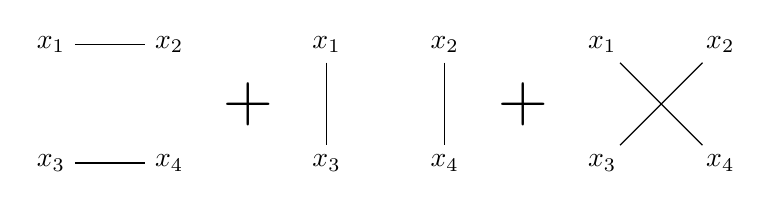
\begin{tikzpicture}
  % Diagram 1: x1-x2 and x3-x4
  \begin{feynman}
    \vertex (a1) at (0,1) {\(x_1\)};
    \vertex (a2) at (1.5,1) {\(x_2\)};
    \vertex (a3) at (0,-0.5) {\(x_3\)};
    \vertex (a4) at (1.5,-0.5) {\(x_4\)};
    
    \diagram* {
      (a1) -- (a2),
      (a3) -- (a4),
    };
  \end{feynman}
  
  % Plus sign
  \node at (2.5,0.25) {\Huge $+$};
  
  % Diagram 2: x1-x3 and x2-x4
  \begin{feynman}
    \vertex (b1) at (3.5,1) {\(x_1\)};
    \vertex (b2) at (5,1) {\(x_2\)};
    \vertex (b3) at (3.5,-0.5) {\(x_3\)};
    \vertex (b4) at (5,-0.5) {\(x_4\)};
    
    \diagram* {
      (b1) -- (b3),
      (b2) -- (b4),
    };
  \end{feynman}
  
  % Plus sign
  \node at (6,0.25) {\Huge $+$};
  
  % Diagram 3: x1-x4 and x2-x3
  \begin{feynman}
    \vertex (c1) at (7,1) {\(x_1\)};
    \vertex (c2) at (8.5,1) {\(x_2\)};
    \vertex (c3) at (7,-0.5) {\(x_3\)};
    \vertex (c4) at (8.5,-0.5) {\(x_4\)};
    
    \diagram* {
      (c1) -- (c4),
      (c2) -- (c3),
    };
  \end{feynman}
\end{tikzpicture}

\vspace{1cm}
Cherchons maintenant un diagramme à une boucle issu du second terme de l'équation (5)
Soit son expression:
\begin{equation}
   - i\frac{\lambda}{4!}\int d^{4}z \bra{0}\mathcal{T}\{\phi^{4}(z)\phi(x_{1})
   \phi(x_{2})\phi(x_{3})\phi(x_{4})\}\ket{0}
\end{equation}  

Une contraction possible est de contracter deux champs en \(z\) entre eux pour former une boucle,
et de contracter les autres champs en \(z\) avec les champs externes \(\phi(x_{1})\)et
\(\phi(x_{2})\), et finalement de contracter \(\phi(x_{3})\) et \(\phi(x_{4})\).

Ce qui en expression donne:
\begin{equation}
    - i\frac{\lambda}{4!}\int d^{4}z \Delta_{F}(z-z)
    \Delta_{F}(z-x_{1})\Delta_{F}(z-x_{2})
    \Delta_{F}(x_{3}-x_{4})
\end{equation}

En diagramme de Feynman, cela se représente comme suit:
\newline
\vspace{1cm}
\begin{tikzpicture}
  \begin{feynman}
    % External points
    \vertex (x1) at (0,1.5) {\(x_1\)};
    \vertex (x2) at (4,1.5) {\(x_2\)};
    \vertex (x3) at (0,-1) {\(x_3\)};
    \vertex (x4) at (4,-1) {\(x_4\)};
    
    % Point z and loop
    \vertex (z) at (2,1.5);
    \vertex (ztop) at (2,2.8);
    
    \diagram* {
      % Line from x1 to z to x2 with loop at z
      (x1) -- (z),
      (z) -- (x2),
      (z) -- [out=90, in=180] (ztop),
      (ztop) -- [out=0, in=90] (z),
      % Simple line connecting x3 and x4
      (x3) -- (x4),
    };
    
    % Label point z
    \node at (2,1) {\(z\)};
  \end{feynman}
\end{tikzpicture}

Ce qui est un diagramme à une boucle contribuant à la fonction de corrélation donnée.







\end{document}
